\documentclass[11pt]{scrartcl}
\usepackage{answers}
\Newassociation{sketch}{hintitem}{hints}
\renewcommand{\solutionextension}{out}
\usepackage{outlines}
\usepackage[sexy]{evan}
\newcommand\EE{\mathbb E}
\newcommand\PP{\mathbb P}
\usepackage{algorithm,algorithmicx,algpseudocode}
\usepackage{graphicx}
\usepackage{wrapfig}
\usepackage[style=ieee]{biblatex}
\addbibresource{refs.bib}

\usepackage{minted} 

\begin{document}
\title{Image Depth Estimation Using Stereo Vision}
\author{Mrinall Umasudhan}
\date{\today}
\maketitle
\Opensolutionfile{hints}

  \noindent Word Count: \mailto{3986},
  Advisor: David Sushil \\ 
  Research Question: To what extent can optimization techniques improve the accuracy and 
  efficiency of pixel correspondence algorithms and stereo vision systems?
 
%TOC
\tableofcontents

% EV.pdf
% ploh handouts



\section{Introduction}
One of the most explored problems in the field of computer vision is the process
of accurately estimating the real-world depth of a pixel within a two-dimensional
image. The inference of three-dimensional information is done by using multiple two-dimensional views of a scene, the process being deemed the name stereo vision.
\subsection{Applications}
A common counter-argument to the practicality of stereo vision algorithms are the presence of other sensors that do not make use of visual data such
as ultrasonic or time of flight distance sensors. While these sensors are not
not impacted by factors that would be detrimental to the accuracy of stereo
vision algorithms such as the lack of adequate lighting,
``stereo vision has the advantage that it achieves the 3-D acquisition without
energy emission or moving parts" (CSIRO). Moreover,
whereas traditional distance sensors focus on a singular point in space, stereo vision
algorithms are only limited by the camera's field of view, making the depth analysis
of a large area far more straightforward and cost effective. Finally, stereo vision algorithms are able
to easily work in conjunction with other
computer vision techniques such as machine learning-based object detection
models, when compared to the previous depth estimation approaches as it operates under the same image plane that a object detection model may be used on, eliminating the need for sensor data conversion.
These factors allow for a more streamlined analysis of the
various shapes and angles in an image leading to its usage in various fields.
\\
\begin{wrapfigure}{R}{0.5\textwidth}
  \centering
  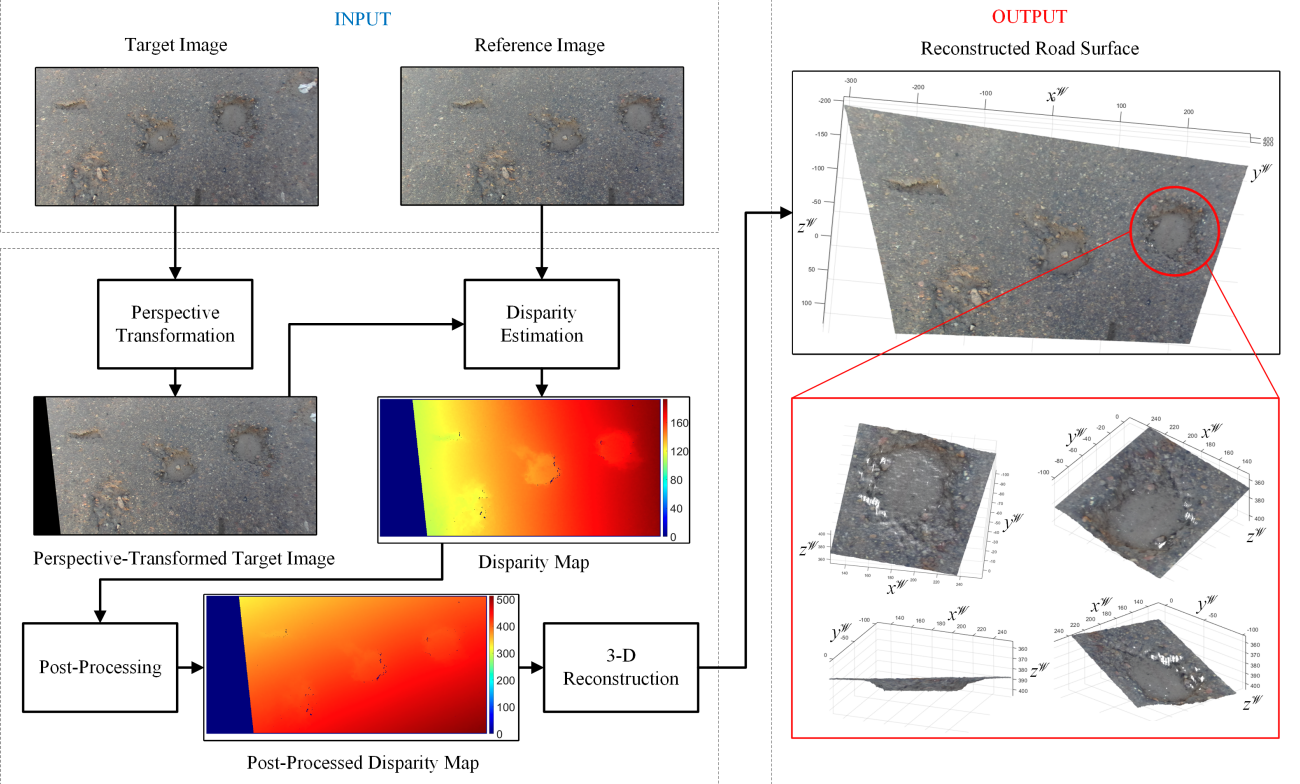
\includegraphics[width=0.5\textwidth]{img1.png}
  \caption{\label{fig:frog1}Stereo Vision For Road Deformity Detection (Rui)}
\end{wrapfigure}

A standard application of stereo vision can be found in the quality
management process of industrial factories. Factories must analyze each
finished products for deformities to maintain a standard of quality in their
products. However, due to the large amounts of product produced, 
manual inspection of each product would be far too expensive and inefficient considering the large amounts of workers required. The installation of multiple
distance sensors to analyze each square inch of a product would also be far too expensive.
However, a factory is a controlled environment with uniform lighting and contains objects
of known shape, the usage of a stereo vision algorithm would be ideal for the situation. Indeed, many factories use this approach rather than spending large sums of money on expensive sensors making use of the camera's wide field of view. 
 \\

Moreover, stereo algorithms hold value outside controlled environments. A paper by the University of Bristol explores this by creating a deformity analysis algorithm  to acquire three-dimensional road data for autonomous cars, further displaying the
capabilities of stereo algorithms. The process that this algorithm follows is illustrated by
figure above.

\subsection{Overview and Purpose}

The essence of a successful stereo vision algorithm can be summarized in three key steps:

  \paragraph{ Triangulation} The Process of assigning depth values to each pixel in the image
        using multiple two-dimensional views of a scene and the specific parameters from
        camera hardware, the difference in the location of the cameras used, and the disparity in the
        pixels from each view of the scene.
    \paragraph{ Calibration}  The process of correcting image distortion that is caused by the
        spherical geometry of the camera lens
        and reifying the two-dimensional views of the scene such that
the views are displayed on the same image plane. 
  \paragraph{Pixel Correspondence} In order to apply the triangulation process, the algorithm must be
        able to match a pixel from one viewpoint of the scene to another viewpoint taken from a separate camera
        also known as the disparity value of this pixel.
\\

\\

In modern research, the most studied step of the algorithm is the process of pixel Correspondence, better known as stereo matching. As of now, researchers are attempting to integrate optimization techniques with stereo matching in order to improve stereo system performance. This paper seeks to provide an in-depth explanation of the stereo vision process in general and find value in the application of optimization techniques to stereo matching algorithms. In order to analyze and implement a sound stereo vision algorithm
as well as an optimized matching algorithm, scholarly sources involving stereo vision and optimization techniques were studied. After implementing a standard stereo matching algorithm and an algorithm that involves a famous optimization technique known as Dynamic Programming, I found that there was a significant increase
in both accuracy and efficiency in the depth estimates provided by the algorithm.


\section{Triangulation}

The core of every stereo vision algorithm is to find the depth of a pixel using multiple two-dimensional views of the scene, more formally this process is known as the backward projection of a camera from image coordinates into three-dimensional world coordinates. In order to derive the formulas for the backward projection model of a camera, the forward projection from scene to image point must be understood. 
\subsection{Forward Projection Model}

Formally defined, the forward projection model ``describes the mathematical relationship
between the coordinates of a point in three-dimensional space and its projection onto the image plane with a ideal pinhole camera, where the camera aperture is described as a point and no lenses are used to focus light" (Maamir, 135). The usage of a pinhole camera allows
for the elimination of lens distortion when mapping to the image plane, simplifying the formulas significantly.

\begin{remark}
  The majority of cameras are used in stereo vision algorithms, including those
  used in this paper, use lenses contradicting the pinhole camera model.
  However, because researchers calibrate their camera's to remove
  distortion from the images returned, the pinhole camera model can still
  be applied.
\end{remark}
The forward projection model of converting a 3D camera point into a 2D pixel
coordinate is defined using the formula below:
\begin{theorem}
  [Forward Projection Equation]

  \begin{displaymath}
    (u, v) = (f_x \cdot \displaystyle\frac{x_c}{z_c} + o_x,
    f_y \cdot \displaystyle\frac{y_c}{z_c} + o_y)
  \end{displaymath}
  \begin{figurekey}
    \begin{tabular}{llll}
      $(u,v)$ & two dimensional pixel coordinates        & $f_x$ & focal length on x-axis \\
      $x_c$   & $x$ position on scene coordinate frame   & $f_y$ & focal length on y-axis \\
      $y_c$   & $y$ position in scene coordinate frame   & $o_x$ & image center on x-axis \\
      $z_c$   & depth of point in scene coordinate frame & $o_y$ & image center on y-axis \\
    \end{tabular}
  \end{figurekey}
  \\ \\ \\
  Equations found in source 5.
\end{theorem}
Whereas the other parameters of the equation are self-explanatory, the focal
length ($f$) requires further explanation. The focal length is ``the distance
between the lens and the image sensor when the subject is in focus" (Berkenfeld).
As such, using this information, the forward projection equations essentially show how a ray from the camera to the scene can be mapped to an image.

\subsection{Derivation of Backwards Projection Model}
It is clear that deriving the depth of a pixel from manipulating the forward
projection equations is impossible given the inquality in depth measurements
when using the $x$ and $y$ pixels. Therefore it is evident that additional
information is needed in order to infer depth. This is where the usage of
multiple viewpoints of a scene is needed.

\begin{remark}
  Although many stereo vision systems use more than two viewpoints of a scene,
  in order to simplify the implementation process a simple (binocular) stereo
  system will be used.
\end{remark}
\begin{wrapfigure}{R}{0.5\textwidth}
  \centering
  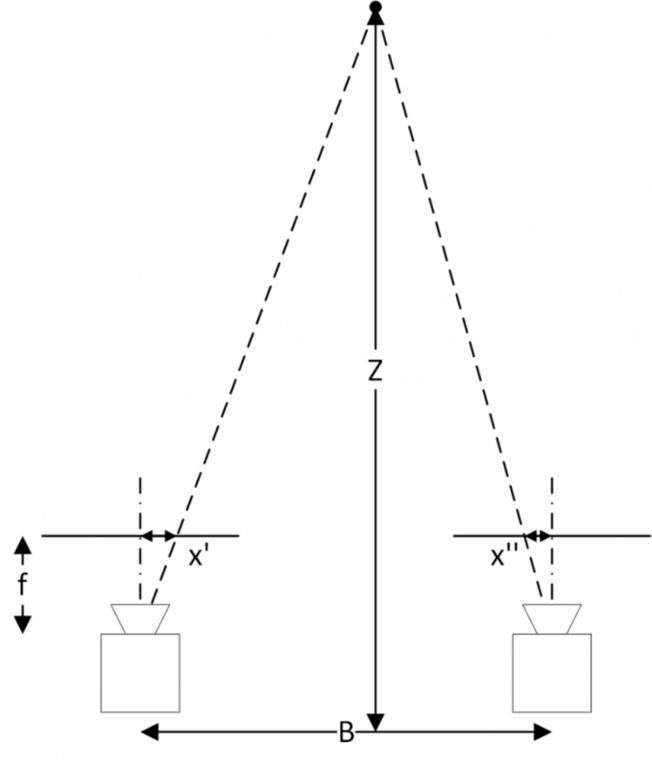
\includegraphics[width=0.3\textwidth]{img2.resized.png}
  \caption{\label{fig:frog2}Simple stereo system}
\end{wrapfigure}
\\
\\

As mentioned prior the forward projection equations essentially represent the camera
as projecting a ray from the image into a scene point. Using this fact, an
additional camera which is calibrated to be on the same plane as the original camera
may be used to project another ray from the corresponding image point onto the scene. By
finding the intersection of these two rays the depth of a pixel in the scene may be found. Using the depth measurement of a pixel, it is also possible to derive
$(x, y)$ coordinates of a scene from the image coordinate frame, giving
the full scene coordinate frame:

\begin{theorem}
  [Backward Projection Equations]

  \begin{align}
    z & = \displaystyle\frac{b\cdot f_x}{(u_r-u_l)} \\
    x & = \displaystyle\frac{z}{f_x} \cdot (u_l - o_x) \\
    y & = \displaystyle\frac{z}{f_y} \cdot (v_l - o_y) 
  \end{align}

  \begin{figurekey}
    \begin{tabular}{llll}
      $(u_l,v_l)$ & pixel coordinates on left camera     & $f_x$ & focal length on x-axis \\
      $(u_r,v_r)$ & pixel coordinates on right camera   & $f_y$ & focal length on y-axis \\
      $x$     & $x$ position on scene coordinate frame  & $o_x$ & image center on x-axis \\
      $y$     & $y$ position in scene coordinate frame   & $o_y$ & image center on y-axis \\
        $z$     & depth of point in scene coordinate frame  &$b$ & baseline distance \\
    \end{tabular}
  \end{figurekey} \\ \\
    Note that the pixel coordinates in the left and right camera point at the same object in 
    the scene. However, because the cameras are located $b$ units away from each other, 
    the coordinates are not equal. The process of finding the corresponding pixel in the 
    right camera for every pixel in the left camera, is known as the stereo correspondence 
    problem. Equations found in source 6. 
\end{theorem}

The two rays projected from the camera, along with the calibrated baseline measurement, distance between the left and right cameras, form a triangle, allowing for the derivations of the formulas
shown above. However, to attain the parameters in these formulas that are not immediately present in the image such as focal length and baseline as well as correcting lens distortion, camera calibration is required. Moreover, to make use of the ray projected from the additional viewpoint, the corresponding pixel from the right camera must be 
found, this can be seen in the calculation of the depth as the $x$ value of the selected pixel in the right camera is subtracted by the $x$ value of the corresponding pixel of the left camera, this value is formally known as the disparity of a pixel $(u_r-u_l)$ and is essential to depth computation. 




\section{Camera Calibration}

For the triangulation formulas to apply all cameras in the stereo 
system must be calibrated to match the pinhole camera model. This involves finding the hardware parameters of the camera and correcting the images returned for lens distortion. Moreover, the images must be transformed such that they are displayed parallel to each other. 

\subsection{Intrinsic matrix}

A key step in correcting for lens distortion and applying the triangulation formulas is identifying the intrinsic parameters of both cameras. Formally explained, the intrinsic parameters are the variables used in the forward projection equations to map 3D scene coordinates into image coordinates, such as the focal length and optical center of the image. The intrinsic parameters of a camera are mathematically contained in 
a 3 by 3 matrix known as the intrinsic matrix. The forward projection equation can be rewritten in matrix form to show this:
 
\begin{theorem}[Forward Projection Equation Matrix Variation]
     \begin{displaymath}
    \begin{bmatrix}
      u \\
      v \\
      w    \end{bmatrix} =
    \begin{bmatrix}
      f_x & 0 & o_x \\
      0 & f_y & o_y \\
      0 & 0 & 1
    \end{bmatrix}
    \begin{bmatrix}
      X \\
      Y \\
      Z
    \end{bmatrix} 
  \end{displaymath}
  \begin{figurekey}
    \begin{tabular}{llll}
      $(u,v)$ & two dimensional pixel coordinates        & $f_x$ & focal length on x-axis \\
      $X$   & $x$ position on scene coordinate frame   & $f_y$ & focal length on y-axis \\
      $Y$   & $y$ position in scene coordinate frame   & $o_x$ & image center on x-axis \\
      $Z$   & depth of point in scene coordinate frame & $o_y$ & image center on y-axis \\
    \end{tabular}
  \end{figurekey}

\end{theorem}


The parameters of the intrinsic matrix can be found by making use of the field of view and resolution of the camera, typically stated in the hardware specifications of the camera. The 
formulas are described below: 

\begin{theorem}
  [Intrinsic Matrix Calculation]

  \begin{align}
      f_x & = \displaystyle\frac{o_x}{\tan{\displaystyle\frac{a_x}{2}}} \\
    f_y & = \displaystyle\frac{o_y}{\tan{\displaystyle\frac{a_y}{2}}}  \\
    o_x & = \displaystyle\frac{r_x}{2} \\ 
    o_y & = \displaystyle\frac{r_y}{2} \\ 
  \end{align}

  \begin{figurekey}
    \begin{tabular}{llll}
      $(u_l,v_l)$ & pixel coordinates on left camera     & $f_x$ & focal length on x-axis \\
      $(u_r,v_r)$ & pixel coordinates on right camera   & $f_y$ & focal length on y-axis \\
      $x$     & $x$ position on scene coordinate frame  & $o_x$ & image center on x-axis \\
      $y$     & $y$ position in scene coordinate frame   & $o_y$ & image center on y-axis \\
        $z$     & depth of point in scene coordinate frame  &$b$ & baseline distance \\
        $a_x$ & horizontal field of view & $a_y$ & vertical field of view \\   
    \end{tabular}
  \end{figurekey} \\ \\
    Note that the pixel coordinates in the left and right camera point at the same object in 
    the scene. However, because the cameras are located $b$ units away from each other, 
    the coordinates are unique creating the pixel correspondence problem. Equations found in source 11.
\end{theorem}



\subsection{Extrinsic Parameters}

The extrinsic parameters of a camera refer to the position and orientation of the camera 
with respect to the world coordinate frame and corresponding cameras. In more complex 
stereo systems an extrinsic matrix is required, detailing the translation of the camera 
in the $x$, $y$, and $z$ axis as well as the roll, pitch, and yaw angles of the cameras. 
However, because a binocular stereo system is used, the two cameras are guaranteed to 
be pointing in a straight line, while being on the same $y$ and $z$ axis leaving only 
a horizontal distance that can easily be manually computed. The baseline ($b$) is measured 
by finding the distance between the centers of the left and rightmost camera. 

\begin{remark}
    Because a simple stereo is used, the cameras are guaranteed to be positioned such the $y$ position of the camera is identical, removing the need for additional calibration beyond the manual baseline measurement. Equations found in source 11. 
\end{remark}

\subsection{Lens Distortion}
    %Images from: https://www.tangramvision.com/blog/camera-modeling-exploring-distortion-and-distortion-models-part-i#tangential-de-centering-distortions
     %Text from: https://docs.opencv.org/4.x/dc/dbb/tutorial_py_calibration.html  
The simple stereo model assumes that both cameras in use do not contain lenses. However, in real-world situations lenses must be present in order to ensure pixel quality. This results in two types of distortion, which must be accounted for when calibrating cameras.  
\paragraph{Radial Distortion}
    This variation of distortion causes ``straight lines in images to appear curved". Moreover, as pixels begin to deviate from the image center, distortion increases rapidly, causing significant drops in accuracy when querying depth (OpenCV). 
\paragraph{Tangential Distortion}
    As opposed to radial distortion, tangential distortion causes some areas in the image to ``appear closer than others due to the misalignment of the lens from the image plane" (OpenCV). 
\\
\begin{figure}[!htb]
    \centering
    \subfloat[\centering Radial]{{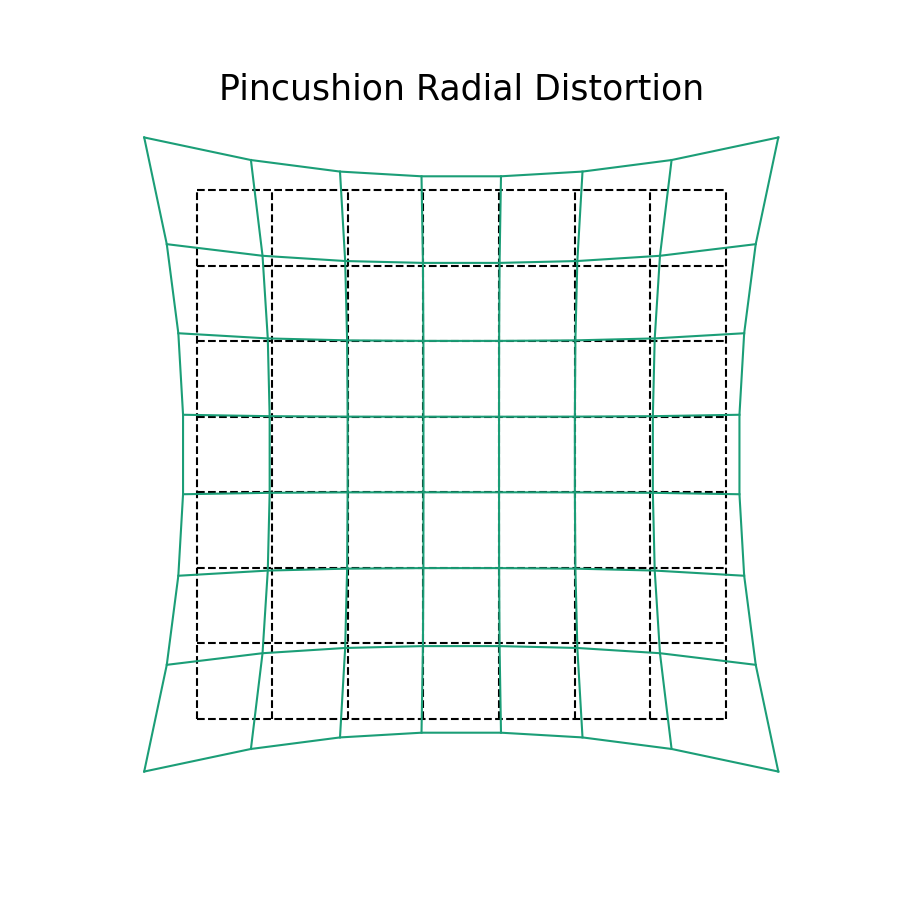
\includegraphics[width=5cm]{radial.png} }}%
    \qquad
    \subfloat[\centering Tangential]{{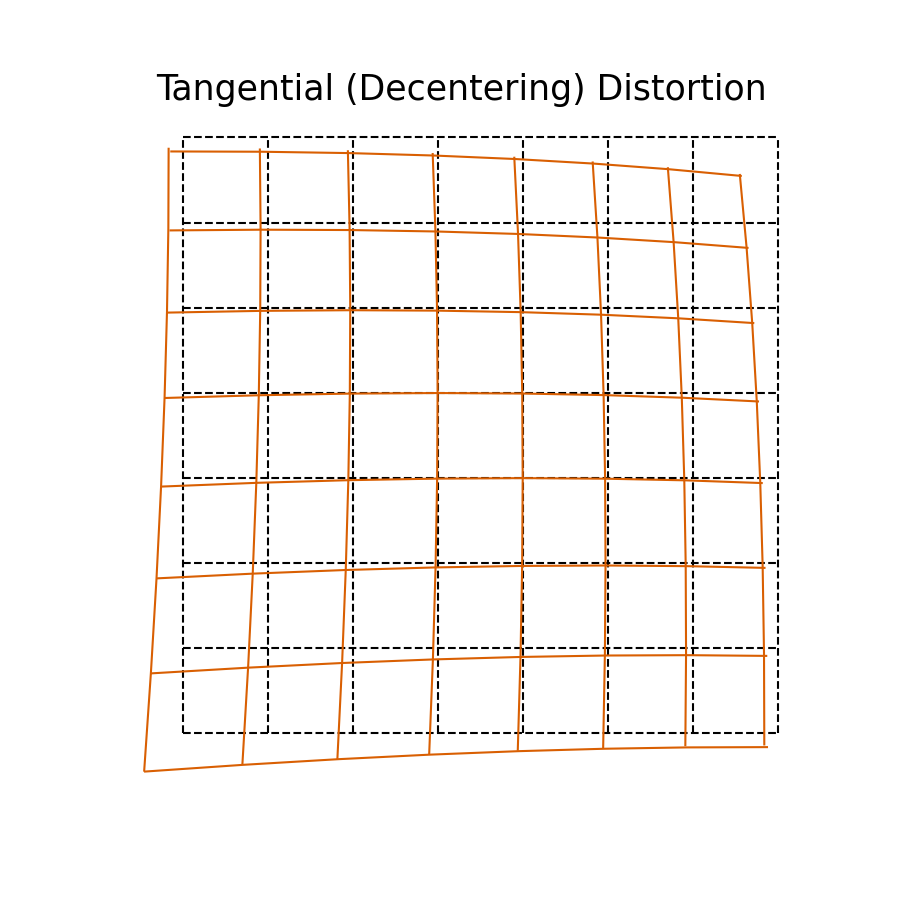
\includegraphics[width=5cm]{tang.png} }}%
    \label{fig:example}% 
    \caption{Impacts of Distortion on the Image Plane (Steward)}
\end{figure}
\\ 

\subsection{Accounting for distortion}

The transformation process between raw and distorted pixels can be modelled using the 
formulas found in the official OpenCV documentation below: 

\begin{theorem}
    [Radial Distortion Equations] 
    \begin{align}
    x_{distorted} = x( 1 + k_1 r^2 + k_2 r^4 + k_3 r^6) 
    \\ y_{distorted} = y( 1 + k_1 r^2 + k_2 r^4 + k_3 r^6)    
    \end{align}
    
\end{theorem}


\begin{theorem}
    [Tangential Distortion Equations] 
    \begin{align}
        x_{distorted} = x + [ 2p_1xy + p_2(r^2+2x^2)]  
       \\ y_{distorted} = y + [ p_1(r^2+ 2y^2)+ 2p_2xy]
    \end{align}
    
\end{theorem}

As seen in the formulas the distortion is magnified through the following distortion coefficients: 
\begin{displaymath}
    Distortion \; coefficients=(k_1 \hspace{10pt} k_2 \hspace{10pt} p_1 \hspace{10pt} p_2 \hspace{10pt} k_3)
\end{displaymath}

By finding these components and transforming the pixels accordingly, the cameras are then completely calibrated. They are found by analyzing multiple images of known geometry and comparing the pixels in the camera with the real-world coordinates of the image. However, 
instead of completing this process manually, OpenCV, the framework being used, automates this process through built-in functions, meaning only a conceptual understanding of lens distortion is needed to proceed. 

\section{Pixel Correspondence}

As mentioned prior, the pixel correspondence problem is the most studied in the field of stereo vision and by extension, the main focus of this paper. The correspondence problem boils down to iterating through each pixel in the left camera and finding the corresponding pixel in the right camera in an efficient and accurate manner. In this paper, 
two methods will be analyzed: a standard window-based approach as well as a newer approach using an optimization technique known as Dynamic Programming (DP) which in theory will increase the program's accuracy and run-time. After implementation, the two approaches will both be tested using the same stereo system in order to reveal differences in accuracy and speed in order to determine the value in the usage of optimization algorithms, such as DP in stereo vision. 

\subsection{Window Based SSD Disparity Estimation}
This method of finding corresponding pixels in two cameras uses a window-based approach. Formally defined a window consists of a $n$ by $n$ grid of pixels. In order to find the corresponding pixel in another camera, the algorithm creates a fixed window centered around the chosen pixel. 
Then on the corresponding row of the second camera, another window is created; however, 
this window is not fixed, rather the algorithm slides the window over every other pixel on the row of the second image. The window that is most similar to the fixed window of the first camera is noted at the corresponding pixel. This process is then repeated for each pixel in the image in order to apply the triangulation formulas and calculate the 
real-world depth of the scene. 
\\
\\
\newpage
Rather than directly comparing individual pixels, the usage of a window of pixels is less resistant to noise and has enough variation to form a pattern, especially when two individual pixels may easily have the same value. The image below shows the window iteration and comparison process described above:

\begin{figure}[!htb]
    \centering
    \subfloat{{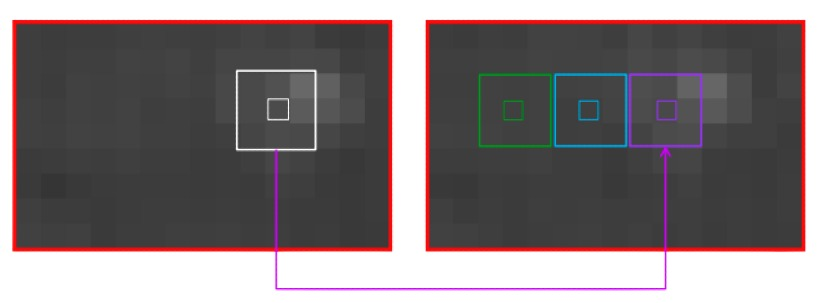
\includegraphics[width=12cm]{SSD.jpg} }}%
    \caption{Window Based Correspondence Illustration (Veksler)}
\end{figure}


\begin{remark}
    Because the cameras have been calibrated, the two images are guaranteed to lie 
    on the same y-axis, therefore the window only needs be transformed in one 
    direction. 
  % https://www.csd.uwo.ca/~oveksler/Courses/Winter2016/CS4442_9542b/L11-CV-stereo.pdf
\end{remark}
\\

\begin{wrapfigure}{R}{0.45\textwidth}
  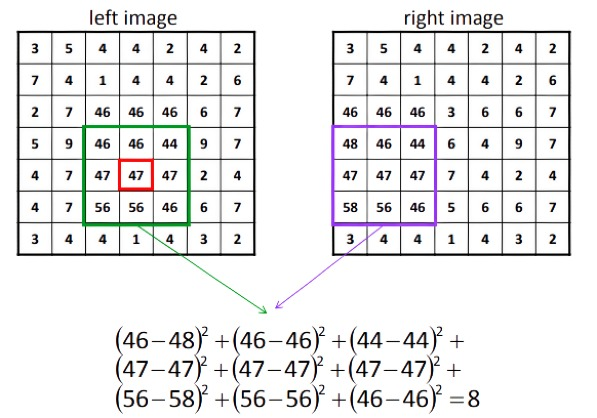
\includegraphics[width=0.6\textwidth]{ex.jpg}
  \caption{\label{fig:frog1} Sample Window Cost Calculation (Veksler)}
\end{wrapfigure}

One segment of the algorithm that has not been explained is how the similarity is measured between two windows. First, the image must be converted from the standard RGB format, a full colored image with each pixel consisting of three color channels: red, green, and blue,  
into a grey-scale image. This is done such that each pixel is normalized from a value between 0 and 255, representing the intensity of light shining on each pixel, so that mathematical operations can be performed easily without having to worry about the additional complexity created by accounting for three color channels. After this, the algorithm makes use of a sum of squared differences approach (SSD) to the windows, in which the squared difference is taken from each pixel in both windows. These differences are then summed up and stored for the pixel centered in the right camera window. The pixel on the right camera with the minimum cost is marked as the corresponding pixel for the pixel centered in the fixed window of the left camera. The cost computation process between the two windows on the left and right images described above is shown by the illustration on the right: 
\newpage

The window iteration process and cost computation method are applied to each pixel in the 
left image in order to attain a disparity map, a map linking each pixel in the left image 
to the corresponding pixel in the right image, is created. This process can be seen in the 
psuedocode below:
\begin{remark}
    The psuedocode below assumes a 3 by 3 window size as the code that will 
    be used to analyze performance will utilize the same dimensions. 
\end{remark}
\begin{algorithm}[!htb]
    \floatname{algorithm}{Window Based Stereo Matching}
    \algrenewcommand\algorithmicrequire{\textbf{Input: image, rows, columns }}
    \algrenewcommand\algorithmicensure{\textbf{Output: disparityMap}}
    \caption{}
    \label{alg:}
    \begin{algorithmic}[1]
        \Require $input$
        \Ensure $output$ 
        \State $rows \gets rows-1$
        \State $columns \gets columns-1$
        \While{$rows \neq 0$}
            \State $curCollumn \gets 1$
            \While{$curCollumn \neq columns$}
                \State $minimmumCost \gets \infty$
                \State $correspondingPixel \gets -1$
                \State $slidingWindow \gets 1$
                \While{$slidingWindow \neq columns$}
                      \State $cost \gets getCost(rows, slidingWindow, curCollumn)$
                      \If{$cost < minimmumCost$}
                         \State $minimmumCost \gets cost$
                         \State $correspondingPixel \gets curCollumn$
                      \EndIf
                \EndWhile
            \EndWhile 
            \State $disparityMap[rows][curCollumn] = correspondingPixel - curCollumn$
        \EndWhile
        \State \textbf{return} $disparityMap$
    \end{algorithmic}
\end{algorithm}

\subsubsection{Drawbacks}
% https://www.researchgate.net/publication/3192330_A_stereo_matching_algorithm_with_an_adaptive_window_Theory_and_experiment
% image from https://www.csd.uwo.ca/~oveksler/Courses/Winter2013/CS4442_9542b/L14-CV-stereo.pdf
\begin{wrapfigure}{R}{0.5\textwidth}
  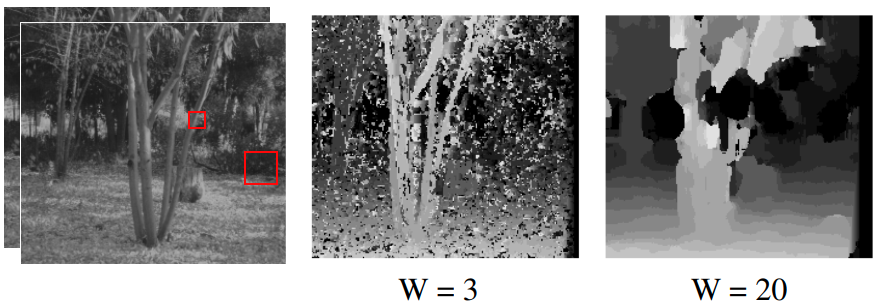
\includegraphics[width=0.7\textwidth]{winsize.png}
    \caption{\label{fig:frog1} Window size compared to depth map (darker pixel shade refers to greater depth) (Olga)}

\end{wrapfigure}


While this algorithm is easy to implement and offers a reasonable amount of accuracy, there are multiple shortcomings to the usage of this method. Firstly, creating multiple windows across images as well as iterating through multiple windows may take a significant amount of processing time, especially as the resolution of the input image increases. Moreover, making use of windows creates a problem 
known as the window sizing problem. Formally defined, ``the window problem states that the window size must be large enough to include enough intensity variation for reliable matching, but small enough to avoid the effects of projective distortion" (Takaeo). This means that when the 
window size is too small, an inaccurate disparity measurement is given as the window does not account for differences in lighting around the pixel which may have significant effects on the cost function. On the other hand, when the window size is too large the disparity measurement may become inaccurate as it ignores the finer details in images and only gives significance to bigger features. The figure on the right displays the 
effects that a smaller or larger window may have when estimating depth. Finally, there is no method to determine whether a pixel being searched for is occluded or present in both images which may lead to significant errors when computing depth. 

% https://www.youtube.com/watch?v=kxsvG4sSuvA
% http://www.cs.umd.edu/~djacobs/CMSC426/Slides/stereo_algo.pdf
\subsection{Dynamic Programming Based Disparity Estimation}
As opposed to the previously described window-based SSD algorithm, the DP algorithm makes use of a function that computes a ``cost" of matching two pixels together. By minimizing the sum of this cost function for each pixel in the image, the corresponding pixel is found for every pixel in the image. The minimization process can be described mathematically below:

\begin{theorem}[Cost Function Minimization]
    \begin{align}
        cost & =  (leftPixel - rightPixel)^2 \\
        d & = \displaystyle\sum_{leftPixel=1}^{N} cost(leftPixel,yPixel,disparity)
    \end{align}
    Note that the cost function can be arbitrarily assigned as the algorithm will always minimize the function. In this paper, the cost function will be equal to the differences between pixel intensities will be squared, the same method that the window-based algorithm uses except with the operation being formed on a singular pixel. 
\end{theorem}

% https://www.ri.cmu.edu/pub_files/pub4/ohta_y_1985_1/ohta_y_1985_1.pdf
% http://www.cs.umd.edu/~djacobs/CMSC426/Slides/stereo_algo.pdf
It is known that the sum of the cost function in all pixels must be minimized, but how can 
the algorithm efficiently approach this problem? This is where Dynamic Programming (DP)
must be used. DP is an optimization technique that increases run-time by breaking a general problem into sub-problems.  As mentioned previously, camera calibration guarantees that the corresponding 
pixel in the left camera must be found in the same row in the right image. This allows for the matching problem to transform into a well-known weighted matching problem which is commonly solved by DP. Imagine forming a $n$ by $n$ grid with n representing the vertical resolution of the pixel. This grid contains $n^2$ columns with the cell in the 
$i$th row and the $j$th column containing the cost of matching the $i$th pixel in the left image's row with the $j$th pixel in the right image. By finding the shortest path, the smallest sum of weights, from the bottom left corner to the top right corner of the grid, the best possible matching configuration is found. DP solves this shortest path problem 
by first solving the problem for smaller sub-rectangles of the entire grid. Moreover, because the pixel matchings must be unique, ``a feature in the left image can match to no more than one feature in the right image", and the ordering must be monotonic, meaning that the path cannot move backward and must be moving in a diagonal manner (Cox). The method by which the algorithm constructs the optimal path by making use of previous path calculations from smaller sub-rectangles is shown below: 
\[
    \texttt{dp}[i][j] =
\begin{cases}
    \max(\texttt{dp}[i-1][j], \texttt{dp}[i][j-1]), \texttt{dp}[i-1][j-1]) + intensity[i][j] \\

\end{cases}
\]
\begin{remark}
    Formally explained, the figure above states that given the last cell of the grid 
    is $(i,j)$, the first cell is $(1,1)$, and the path must not have any discontinuities, 
    the second to last cell must be one of the following: $(i-1, j-1)$ , $(i, j-1)$ , or 
    $(i-1, j)$. These options represent the optimal path from a sub-rectangle spanning from $(0,0)$
    to the listed positions. Thus by adding the value of cell $(i, j)$ to the paths ending on the previously mentioned cells, all possible paths ending on $(i,j)$ are constructed. As such, this process of using optimal paths of previous sub-rectangles motivates the statement above. By repeating 
    this process for every pixel in the grid, an optimal matching pattern for every pixel from 
    $(1,1)$ to $(n,n)$. 
\end{remark}

\subsubsection{Advantages}

\begin{wrapfigure}{R}{0.53\textwidth}
  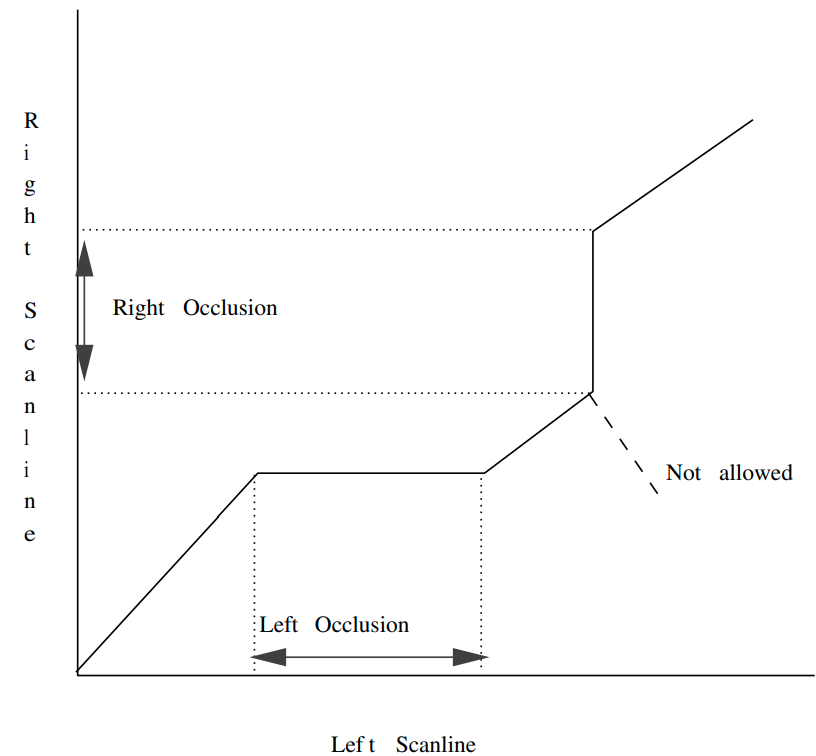
\includegraphics[width=0.5\textwidth]{dpG.png}
    \caption{\label{fig:frog1} Example of optimal pixel matching path found by DP algorithm (Cox)}
\end{wrapfigure}
\\ 
There are many theoretical advantages of implementing
a DP based algorithm over a window based algorithm. 
As previously mentioned, DP allows for the reduction 
of run-time from a polynomial $n^x$ operations into 
a linear $n$ operations due to utilizing individual 
pixel intensities. Moreover, making use of individual pixels 
allows for the circumvention of the window sizing problems 
associated with the SSD based algorithm, increasing accuracy 
significantly. Finally, making use of DP allows the algorithm 
to recognize when a pixel has no reasonable matches. This can be detected 
as a valid path must be diagonal in nature; therefore when the pixel with the 
lowest cost forms a straight line with the pixel in question, the pixel is marked 
as occluded as including the pixel would lead to an unoptimal cost and by extension, 
a unoptimal matching arrangement. The figure to the right illustrates the concept 
of constructing an optimal path while detecting occlusions. 



\section{Implementation}
Now that the general components of the algorithm have been discussed, the implementation 
and testing process can be described. 

\subsection{Tools}

In order to create a rudimentary binocular stereo system, two Logitech C270 webcams will be attached to a wooden apparatus 3 inches apart. The cameras will then be connected to a laptop to execute the program. In regards to the software aspect of implementation, the Python programming language will be used in conjunction with a widely used Computer Vision framework known as OpenCV which allows the program to query image data from both cameras. The overall structure of the code can be explained through the following outline:



\subsection{Testing}
In order to test the algorithm, I created several varying scenes with variable surroundings 
and lighting conditions in order to verify the speed and accuracy of which both correspondence
algorithms preformed when inferring the depth of all objects on the scene. For this paper 
major objects are classified as objects which are of significant size such that they are clearly 
distinct from the background of a image. The figure to the right gives an example of a scene used 
in testing. The outline below illustrates how all of the steps discussed in previous sections 
combine in order to measure performance of the correspondence algorithms in question. 
\begin{outline}[enumerate]
   \1 Query images from left and right cameras.  
    \1 Calculate intrinsic and extrinsic parameters 
   \1 Correct for Image Distortion 
   \1 Start first timer 
   \1 Start first window based stereo correspondence algorithm 
   \1 End timer when correspondence algorithm is finished running and store time taken 
   \1 Start second timer
   \1 Run DP based correspondence algorithm 
   \1 End timer when algorithm is finished running and store time taken
   \1 Measure true accuracy rate compared with a purposefully placed object on the scene 
        to true depth. 
    \1 Store time taken and accuracy rates for data analysis. 
    \1 Repeat for all test cases. 
\end{outline}
\section{Results and Conclusion}

After running the algorithms against 20 various scenes, the following results were 
produced:
\\

\begin{table}[H]
\begin{tabular}{lll}
\hline
Scene & Window Correspondence Runtime (ms) & DP Correspondance Runtime (ms) \\ \hline
1     & 1300                               & 302                            \\
2     & 1173                               & 341                            \\
3     & 1420                               & 629                            \\
4     & 1912                               & 640                            \\
5     & 1341                               & 452                            \\
6     & 1119                               & 501                            \\
7     & 1132                               & 643                            \\
8     & 2016                               & 751                            \\
9     & 1251                               & 364                            \\
10    & 1762                               & 704                            \\ \hline
\end{tabular}
\end{table}

\\
\begin{table}[H]
\begin{tabular}{lll}
\hline
Scene & Window Correspondance Error (in) & DP Correspondance Error (in) \\ \hline
1     & 1.95                             & 0.34                         \\
2     & 2.40                             & 1.12                         \\
3     & 1.33                             & 0.78                         \\
4     & 2.45                             & 0.51                         \\
5     & 1.50                             & 1.20                         \\
6     & 2.04                             & 0.83                         \\
7     & 2.09                             & 1.33                         \\
8     & 2.41                             & 0.35                         \\
9     & 1.41                             & 0.47                         \\
10    & 2.27                             & 1.20                         \\ \hline
\end{tabular}
\end{table}

All in all, the results show that the DP-based algorithm offers significantly lower runtimes while returning a more accurate depth measurement compared to the window-based algorithm. The results align with the theoretical conclusion that a DP-based approach is superior to the standard method. However, the DP solution did not eliminate computation errors. These errors may have been caused by inaccuracies in measurement when verifying the true distance or when manually entering extrinsic parameters such as the baseline measurement. Another possible explanation of such error may be associated with the issue of making use of a stereo algorithm in which variations of lighting cause misinterpretations of the cost function. As such, additional questions regarding the validity of stereo systems as a whole can be brought into question. There may be better methods of estimating image depth such as matching external sensor data with image pixels, such as cutting-edge LiDAR sensors. Regardless, stereo vision systems are able to offer low-cost solutions to depth estimation in many situations and with the added value of optimization techniques such as DP, stereo systems continue to be a feasible solution for attaining 3D understanding from images.  



\section{Appendix}

\subsection{Query Image Data}
\begin{minted}{python}
# query image data
cam1 = cv2.VideoCapture(0)
cam2 = cv2.VideoCapture(1)
ret1, frame1 = cam1.read()
ret2, frame2 = cam2.read()
\end{minted}

\subsection{Camera Calibration}
\begin{minted}{python}
# Returns intrinsic and extrinsic parameters along with undistorted images
def calibrateCamera(f, leftImg, rightImg, xResolution, yResolution):
    calibrationResults = []
    # Manually Computed Parameters
    a_x = 45
    a_y = 45
    o_x = xResolution / 2
    o_y = yResolution / 2
    f_x = o_x / (math.tan(a_x / 2))
    f_y = o_y / (math.tan(a_y / 2))
    calibrationResults.append(f_x)
    calibrationResults.append(f_y)
    calibrationResults.append(o_x)
    calibrationResults.append(o_y)

    # Following lines are from official OPENCV Documentation for Camera Calibration

    # termination criteria
    criteria = (cv2.TERM_CRITERIA_EPS + cv2.TERM_CRITERIA_MAX_ITER, 30, 0.001)
    # prepare object points, like (0,0,0), (1,0,0), (2,0,0) ....,(6,5,0)
    objp = np.zeros((6 * 7, 3), np.float32)
    objp[:, :2] = np.mgrid[0:7, 0:6].T.reshape(-1, 2)
    # Arrays to store object points and image points from all the images.
    objpoints = []  # 3d point in real world space
    imgpoints = []  # 2d points in image plane.
    images = glob.glob('leftCam.jpg')
    for fname in images:
        img = cv2.imread(fname)
        gray = cv2.cvtColor(img, cv2.COLOR_BGR2GRAY)
        # Find the chess board corners
        ret, corners = cv2.findChessboardCorners(gray, (7, 6), None)
        # If found, add object points, image points (after refining them)
        if ret == True:
            objpoints.append(objp)
            corners2 = cv2.cornerSubPix(gray, corners, (11, 11), (-1, -1), criteria)
            imgpoints.append(corners)
            # Draw and display the corners
            cv2.drawChessboardCorners(img, (7, 6), corners2, ret)
            cv2.imshow('img', img)
            cv2.waitKey(500)
    ret, mtx, dist, rvecs, tvecs = cv2.calibrateCamera(objpoints, imgpoints, 
    gray.shape[::-1], None, None)
    h, w = leftImg.shape[:2]
    newcameramtx, roi = cv2.getOptimalNewCameraMatrix(mtx, dist, (w, h), 1, (w, h))
    img = frame1
    # Undistort
    dst = cv2.undistort(img, mtx, dist, None, newcameramtx)
    # crop the image
    x, y, w, h = roi
    leftImageUndistorted = dst[y:y + h, x:x + w]
    calibrationResults.append(leftImageUndistorted)

    # Repeat for right camera image
    criteria = (cv2.TERM_CRITERIA_EPS + cv2.TERM_CRITERIA_MAX_ITER, 30, 0.001)
    # prepare object points, like (0,0,0), (1,0,0), (2,0,0) ....,(6,5,0)
    objp = np.zeros((6 * 7, 3), np.float32)
    objp[:, :2] = np.mgrid[0:7, 0:6].T.reshape(-1, 2)
    # Arrays to store object points and image points from all the images.
    objpoints = []  # 3d point in real world space
    imgpoints = []  # 2d points in image plane.
    images = glob.glob('rightCam.jpg')
    for fname in images:
        img = cv2.imread(fname)
        gray = cv2.cvtColor(img, cv2.COLOR_BGR2GRAY)
        # Find the chess board corners
        ret, corners = cv2.findChessboardCorners(gray, (7, 6), None)
        # If found, add object points, image points (after refining them)
        if ret == True:
            objpoints.append(objp)
            corners2 = cv2.cornerSubPix(gray, corners, (11, 11), (-1, -1), criteria)
            imgpoints.append(corners)
            # Draw and display the corners
            cv2.drawChessboardCorners(img, (7, 6), corners2, ret)
            cv2.imshow('img', img)
            cv2.waitKey(500)
    img = frame2
    ret, mtx, dist, rvecs, tvecs = cv2.calibrateCamera(objpoints, imgpoints, 
    gray.shape[::-1], None, None)
    h, w = leftImg.shape[:2]
    newcameramtx, roi = cv2.getOptimalNewCameraMatrix(mtx, dist, (w, h), 1, (w, h))
    # Undistort
    dst = cv2.undistort(img, mtx, dist, None, newcameramtx)
    # crop the image
    x, y, w, h = roi
    rightImageUndistorted = dst[y:y + h, x:x + w]
    calibrationResults.append(rightImageUndistorted)

    # returns f_x, f_y, imagecenterx, imagecentery, undistorted left image, 
    #undistorted right image
    return calibrationResults
\end{minted}

\subsection{Depth Calculation}
\begin{minted}{python}
def getDepthMap(xResolution, yResolution, disparityMap, baseline, f_x, f_y):
    output = []
    new = []
    # Initialize Depth Map
    for i in range(1, xResolution):
        for j in range(1, yResolution):
            new.append(0)
        output.append(new)
        new = []
    # Apply Triangulation Equations
    for i in range(1, xResolution):
        for j in range(1, yResolution):
            output[i][j] = (baseline * f_x) / (disparityMap[i][j])
    return output
\end{minted}
\newpage
\subsection{Window Based Correspondence Algorithm}
\begin{minted}{python}
def windowCorrespondance(leftImg, rightImg, rows, columns):
    disparityMap = []
    new = []
    # Initialize Depth Map
    for i in range(1, rows):
        for j in range(1, columns):
            new.append(0)
        disparityMap.append(new)
        new = []
    rows = rows - 1
    columns = columns - 1

    for i in range(1, rows):
        for j in range(1, columns):
            minCost = 1000000000
            matchedPixel = -1
            slidingWindowCenter = 1
            fixedWindow = [[leftImg[i - 1][j - 1], leftImg[i - 1][j], 
            leftImg[i - 1][i + 1]],
                           [leftImg[i][j - 1], leftImg[i][j], leftImg[i][j + 1]],
                           [leftImg[i + 1][j - 1], leftImg[i + 1][j], 
                           leftImg[i + 1][j + 1]]]
            while slidingWindowCenter < columns:
                slidingWindow = [
                    [rightImg[i - 1][slidingWindowCenter - 1], 
                    rightImg[i - 1][slidingWindowCenter],
                     rightImg[i - 1][slidingWindowCenter + 1]],
                    [rightImg[i][slidingWindowCenter - 1], 
                    rightImg[i][slidingWindowCenter],
                     rightImg[i][slidingWindowCenter + 1]],
                    [rightImg[i + 1][slidingWindowCenter - 1], 
                    rightImg[i + 1][slidingWindowCenter],
                     rightImg[i + 1][slidingWindowCenter + 1]]]

                cost = 0
                for k in range(0, 2):
                    for l in range(0, 2):
                        cost += math.pow((fixedWindow[k][l] - slidingWindow[k][l]), 2)
                if minCost > cost:
                    minCost = cost
                    matchedPixel = slidingWindowCenter
                slidingWindowCenter += 1
            disparityMap[i][j] = matchedPixel - j
    return disparityMap
\end{minted}
\newpage
\subsection{Dynamic Programming Based Correspondence Algorithm}
Code Inspired From psuedocode provided in: Cox, Ingemar J., Sunita L. Hingorani, Satish B. Rao, and Bruce M. Maggs. 
"A maximum likelihood stereo algorithm." Computer vision and image understanding 63, 
no. 3 (1996): 542-567.
\begin{minted}{python}
def DynamicProgrammingCorrespondance(leftImage, rightImage, rows, columns):
    cost = np.zeros(rows, columns)  # Fill with zeros
    disparityMap = np.zeros(rows, columns)
    pathTracker = np.zeros(rows, columns)
    occ = 0.0009  # threshold to determine if pixel is occluded
    for row in range(rows - 1):
        # Initialize DP values to be occluded for now
        for i in range(columns - 1):
            cost[1][i] = i * occ
        for i in range(columns - 1):
            cost[i][1] = i * occ
        # Find optimal path for every pixel through dynamic programming
        for i in range(columns - 1):
            for j in range(columns - 1):
                curCost = math.pow(leftImage[row][i] - rightImage[row][j], 2)
                # Find all possible path sums through dynamic programming
                # by using previous answers from smaller rectangles.
                # Invalid paths indicate occluded pixels
                m1 = cost[i - 1][j - 1] + curCost  # Valid diagonal path
                m2 = cost[i - 1][j] + occ  # Invalid Vertical Path
                m3 = cost[i][j - 1] + occ  # Invalid Horizontal Path
                cost[i][j] = min(m1, m2, m3)
                if m1 == cost[i][j]:
                    pathTracker[i][j] = 1  # Pixel can be matched
                elif m2 == cost[i][j]:
                    pathTracker[i][j] = 2  # Pixel is occluded because the occlusion  
                    # cost is lower than matching it
                    # with the most suitable pixel
                else:
                    pathTracker[i][j] = 3  # Pixel is occluded because the occlusion 
                    # cost is lower than matching it
                    # with the most suitable pixel
        # Reconstruct the best possible path by working backwards,
        # and match the pixels which are not occluded
        # meaning pathtracker for the two pixels is equal = 1
        i = columns - 1
        j = columns - 1
        while i >= 0 and j >= 0:
            if pathTracker[i][j] == 1:
                disparityMap[row][j] = abs(i - j)  # Match both pixel to each other
                disparityMap[row][i] = abs(i - j)
                i -= 1  # Continue along the path
                j -= 1
            elif pathTracker[i][j] == 2:
                disparityMap[row][j] = None  # Pixel is occluded 
                #(Path was marked as invalid)
                i -= 1  # Continue along the path
            else:
                disparityMap[row][j] = None  # Pixel is occluded 
                #(Path was marked as invalid)
                j -= 1  # Continue along the path
        # Reset cost and path tracker for subsequent rows
        cost = np.zeros(rows, columns)
        pathTracker = np.zeros(rows, columns)
    return disparityMap
\end{minted}
\section{Works Cited}
\renewcommand{\section}[2]{}%
\begin{thebibliography}{9}

\bibitem{Cox}
Cox, Ingemar J., et al (1996): \emph{A Maximum Likelihood Stereo Algorithm}, Computer vision and image understanding 63.3: 542-567.

\bibitem{Takeo}
Kanade, Takeo & Okutomi, Masatoshi. (1994):  \emph{A stereo matching algorithm with an adaptive window: Theory and experiment}, Pattern Analysis and Machine Intelligence, IEEE Transactions on. 16. 920 - 932. 10.1109/34.310690. 

\bibitem{Maamir}
Maamir, S. and Haghi, A.K. (2015): \emph{Mechanical and Physico-Chemical Characteristics of Modified Materials: Performance}, Apple Academic Press,
ISBN: 9781498714105

\bibitem{Bristol}
Fan, R., Liu, Y., Yang, X., Bocus, J., Dahnoun, N., & Tancock, S. (2018). \emph{Real-Time Stereo Vision for Road Surface 3-D Reconstruction.} In Real-Time Stereo Vision for Road Surface 3-D Reconstruction \url{https://arxiv.org/abs/1807.07433}

\bibitem{Lowe}
David Lowe (2007): \emph{Stereo Vision}, University of British Columbia, CPSC 425: Computer Vision, 
\url{https://www.cs.ubc.ca/~lowe/425/slides/6-Stereo.pdf}

\bibitem{Olga}
Veksler Olga  (2016): \emph{CS4442/9542b Artificial Intelligence II, Lecture 11}, University of Waterloo,
\url{https://www.csd.uwo.ca/~oveksler/Courses/Winter2016/CS4442_9542b/L11-CV-stereo.pdf}

\bibitem{Nayar1}
Shree Nayar (2021): \emph{Camera Calibration | Uncalibrated Stereo}, Columbia University, 
\url{https://www.youtube.com/playlist?list=PL2zRqk16wsdoCCLpou-dGo7QQNks1Ppzo}

\bibitem{CSIRO}
  CSIRO Research,
  \textit{Stereo Vision}, \url{https://research.csiro.au/qi/stereo-vision/}
  
\bibitem{OpenCV}
Open Source Computer Vision (OpenCV): \emph{Camera Calibration},
\url{https://docs.opencv.org/4.x/dc/dbb/tutorial_py_calibration.html}

\bibitem{Nikon}
Diane Berkenfeld et al: \emph{Understanding Focal Length}, Nikon,
\url{https://www.nikonusa.com/en/learn-and-explore/a/tips-and-techniques/understanding-focal-length.html}

\bibitem{stew}Jeremy Steward, Camera Modeling: Exploring Distortion and Distortion Models, Part I, \url{https://www.tangramvision.com/blog/camera-modeling-exploring-distortion-and-distortion-models-part-i#tangential-de-centering-distortions}

\bibitem{bl}Ashwin Nanjappa, How to compute intrinsic camera matrix for a camera, \\
https://codeyarns.com/tech/2015-09-08-how-to-compute-intrinsic-camera-matrix-for-a-camera.html#gsc.tab=0




 
\end{thebibliography}

\end{document}
